\section{Durchführung}
\label{sec:Durchführung}

\subsection{Bestimmung der Schallgeschwindigkeit mittels Impuls-Echo-Verfahren}
Als erstes wird ein Acrylzylinder mit 
einer der \SI{2}{\mega\hertz}-Sonde auf einer Schicht aus bidestiliertem 
Wassser gekoppelt. Damit wird ein A-Scan mittels 
Impuls-Echo-Verfahren durchgeführt. Für die ersten beiden 
Pulse werden die Laufzeit und Amplitude 
gemessen. 
Die Länge des Zylinders wird gemessen.
Diese Messung wird mit vier weiteren Acrylzylinder wiederholt. 

\subsection{Bestimmung der Dämpfung mittels Impuls-Echo-Verfahren}
Aus den vorherigen Messungen wird für alle fünf Acrylzylinder
durch die Amplituden der materialspezifischen Schwächungskoeffizient bestimmt.

\subsection{Bestimmung der Schallgeschwindigkeit mittels Durchschall-Verfahren}
Die Acrylzylinder werden in die Halterung gespannt und an 
beiden Seiten wird jeweils eine Sonde mit Koppelgel gekoppelt. 
Mit einem A-Scan wird die Laufzeit bestimmt, indem die Zeiten
der ersten beiden Amplituden gemessen werden. Die Messung wird für alle 
Zylinder wiederholt.

\subsection{Biometrische Untersuchung eines Augenmodells}
Die \SI{2}{\mega\hertz}-Sonde wird mit Koppelgel auf die
Hornhaut des Augenmodells gesetzt. Mit einem A-Scan werden die
Echos an den Grenzflächen der Iris und der Retina aufgenommen.
Aus den Zeitpunkten können die Abmessungen des Auges bestimmt 
werden.
\begin{figure}
    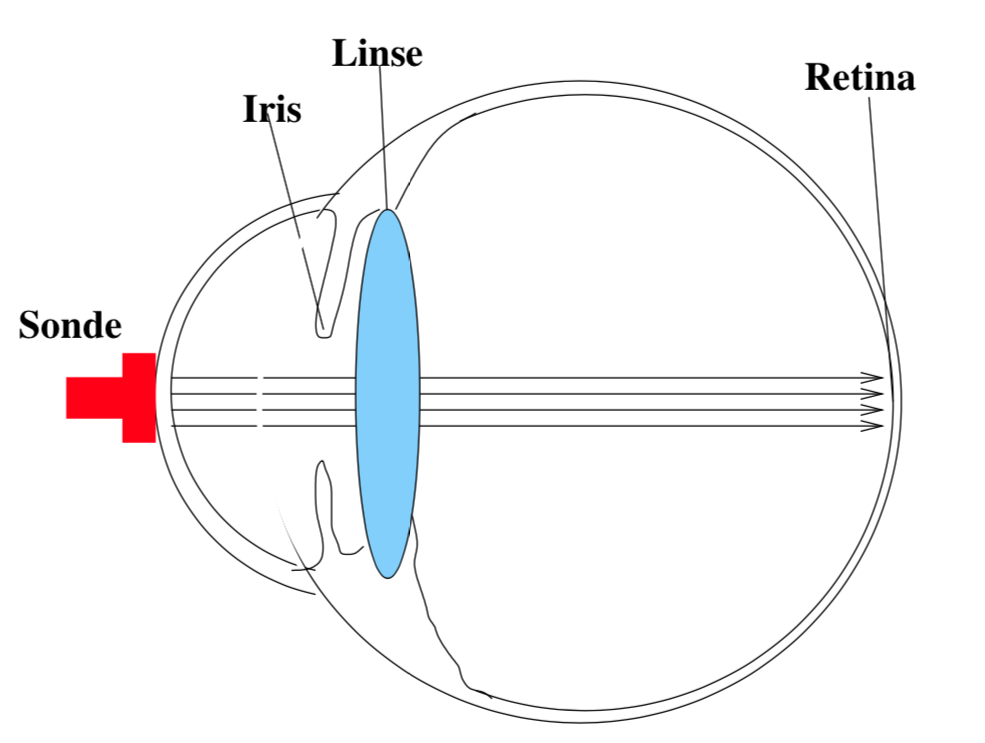
\includegraphics{build\Augenmodell.png}
    \caption{}
    \label{fig:augenmodell}
\end{figure}